\section{Implementation and Results}
\label{sec:implementationandresults}  
%Let us suppose the following medical scenario to illustrate our service-based query rewriting algorithm. 
%Users can access \textit{abstract services} (basic service capabilities) to retrieve: (i) patients infected by a given disease (\textit{DiseasePatients(d?,p!)});
%(ii) patient dna information \textit{PatientDNA(p?, dna!)}; and (iii) patient personal information (\textit{PatientInformation(p?, info!)}).
%To perform these function consider the \textit{abstract services}: (i)
%, (ii)  and (iii)
%.
%The decorations ? and ! are used to specify input and output parameters, respectively. 

%Users can retrieve information about patients, diseases, dna information and others.
%To perform these function consider the \textit{abstract services}: (i)
%\textit{DiseasePatients(d?,p!)}, (ii) \textit{PatientDNA(p?,dna!)} and (iii)
%\textit{PatientInformation(p?,info!)}.
%The decorations ? and ! are used to specify input and output parameters, respectively. 

% 
% \begin{table}[h!]
% \center
% \begin{tabular}{|p{3.7cm}|p{4cm}|}
% \hline
% \begin{small} \textbf{\textit{Abstract Service}} \end{small} & \begin{small}\textbf{\textit{Description}} \end{small}\\ 
% \hline 
% \begin{small} \textit{DiseasePatients(d?,p!)} \end{small} & \begin{small} Given a disease \textit{d}, a list of patients \textit{p} infected by it is retrieved. \end{small}\\ 
% \hline 
% \begin{small} \textit{PatientDNA(p?,dna!)} \end{small} & \begin{small} Given a patient \textit{p}, his DNA information \textit{dna} is retrieved. \end{small}\\ 
% \hline 
% \begin{small} \textit{PatientInformation(p?,info!)} \end{small} & \begin{small} Given a patient \textit{p}, his personal information \textit{info} is retrieved. \end{small}\\ 
% \hline 
% \end{tabular} \caption{List of \textit{abstract services}}
% \end{table}\label{table:abstractservices}

%In our scenario, a \textit{query} expresses an abstract composition that
% describes the requirements of a user.
%\textit{Queries} and \textit{concrete services} are defined in terms of
% \textit{abstract services}.
%They can be associated to a single \textit{abstract service} or to a
% composition of them.

%Let us consider the query: \textit{a user wants to retrieve personal and DNA information of patients who were infected by a disease `K' using services that have availability higher than 98\%, price per call less than 0.2 dollars, and total cost less than 1 dollar.} 
%The query below corresponds to the example (see Definition 1).
% A query $Q$ tagged with user preferences is defined in accordance with the grammar:
% \begin{center}
% $Q (\overline{I}, \overline{O}) := A_{1}(\overline{I}, \overline{O}), A_{2}(\overline{I}, \overline{O}), ..,  A_{n}(\overline{I}, \overline{O})[P_{1},P_{2}, .., P_{k}]$
% \end{center}
% where the left side is the \textit{head} of the query; and the right side is the \textit{body}. 
% $\overline{I}$ and $\overline{O}$ are a set of \textit{input} and \textit{output} parameters, respectively.
% Input parameters present in both sides of the definition are called \textit{head variables}.
% In contrast, input parameters only in the body are called \textit{local variables}.
% $A_{1}, A_{2}, .., A_{n}$ are \textit{abstract services}.
% $P_{1}, P_{2}, .., P_{k}$ are user preferences (over the services). Preferences are in the form $x \otimes constant$ such that $\otimes \in\lbrace \geq, \leq, =, \neq, <, >\rbrace$.

%The query which express the example following our grammar is below.
%The decorations ? and ! are used to specify input and output parameters, respectively. 
%\begin{small}
%\begin{center}
%$Q (d?, dna!) := DiseasePatients(d?, p!), PatientDNA(p?, dna!),$ \\
%$[availability > 99\%, \ price \ per \ call < 0.2\$, \ total \ cost < 1\$]$
%\end{center} 
%\end{small}

%We highlight that in the query there are two types of preferences (let's refer
%to them as \textit{measures}): \textit{single measures} (availability and price
%per call) and \textit{composed measures} (total cost).
%The \textit{single measures} are the simplest type. It is a static measure
% which is has a name associated with an operation and a value. The\textit{ composed measure} is dynamically computed measure. It is defined as aggregations of \textit{single measures}.

%\textit{Concrete services} are defined follwing the same grammar as the
%\textit{query}. The only difference is that concrete services do not have
%\textit{composed measures}. 



% ----- Daniel ----- %   
The Rhone prototype is implemented in Java.
There are 15 classes in which 14 of them model the basic concepts 
(\textit{query}, \textit{abstract services}, \textit{concrete services}, etc), 
and 1 responsible to implement the core of the algorithm.

Currently, our approach runs in a controlled environment. 
Two experiments were produced: \textit{Test 1} and \textit{Test 2}. 
In both the query contains 6 \textit{abstract services} and 4 quality \textit{measures}.
The service registry used has 35 concrete services.

In each experiment, there are a set of tests in which the number of concrete 
services varies from 2 to 35.
The important difference between the experiments is regarding the use of quality preferences
to guide the service selection and query rewriting.
\textit{Test 1} do not consider quality measures. 
On the other hand, \textit{Test 2} consider them.
The figure 1 shows our first results.
  
\begin{figure}[!h]
\centering
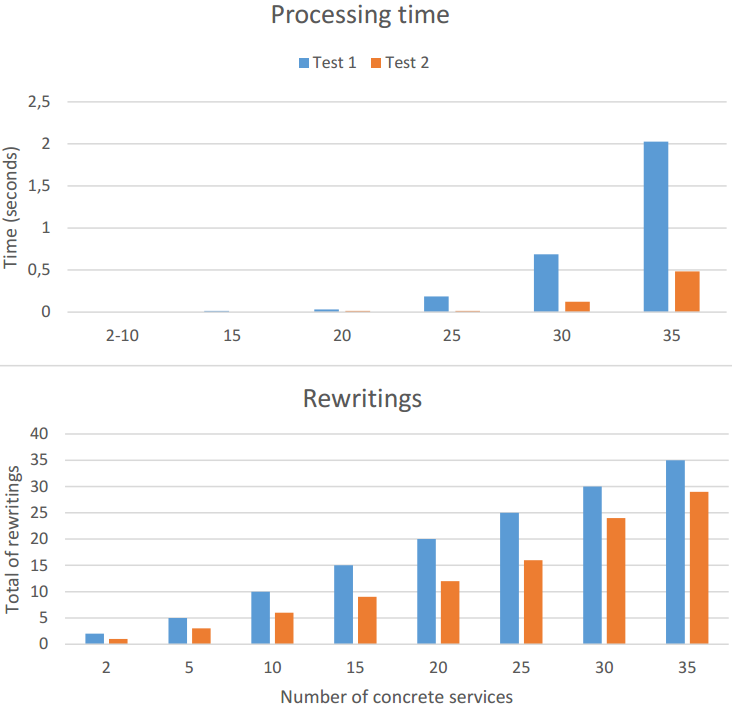
\includegraphics[scale=0.32]{analysis.png}
\label{fig:fig01}
\caption{Query rewriting evaluation.}
\end{figure} 
 
The analysis identified that the algorithm shares the same problem as  existing query rewriting 
approaches using views (database domain) while it does not take into account quality measures (\textit{Test 1}): 
increasing the processing time when the query and the number of concrete services increase. 
However, while considering the quality measures (\textit{Test 2}), the results are promisingly.  
The \textit{Rhone} presents a better performance, decreasing the processing time and 
the total number of rewritings produced.  

%By now, the analysis identified that the factor that influenciates the Rhone
%performance is the number of CSDs versus the number of abstract services in the
%query since they increase the number of possible combinations of CSDs.  
%We proceeded two types of analysis for the query $Q$ (\textit{Test 1} and
%\textit{Test 2} - Figure 1). The first set of tests doesn't consider quality measures,
%while the second consider the measures in the rewriting process. The number of
%concrete services used in the analysis is from 2 until 35 services. Our
%preliminary results show that our algorithm, considering the quality measures,
%presents a better result for performance and the total number of rewritings.    

%To illustrate our approach in the next section, consider the \textit{concrete
% services} in table~\ref{table:concreteservices}.

% \begin{table}[h!]
% \center
% \begin{tabular}{p{7cm}}
% \hline
% \begin{small} $S1 (a?, b!) := DiseaseInfectedPatients(a?, b!)$ \end{small}\\ 
% \begin{small} $[availability > 99\%, \ price \ per \ call = 0.2\$]$ \end{small}\\ 
% \hline 
% \begin{small} $S2 (a?, b!) := DiseaseInfectedPatients(a?, b!)$ \end{small}\\
% \begin{small} $[availability > 99\%, \ price \ per \ call = 0.1\$]$ \end{small}\\ 
% \hline 
% \begin{small} $S3 (a?, b!, c!) := DiseaseInfectedPatients(a?, b!, c!)$ \end{small}\\
% \begin{small} $[availability > 98\%, \ price \ per \ call = 0.1\$]$ \end{small}\\ 
% \hline 
% \begin{small} $S4 (a?, b!) := PatientDNA(a?, b!)$ \end{small}\\
% \begin{small} $[availability > 99.5\%, \ price \ per \ call = 0.1\$]$ \end{small}\\ 
% \hline
% \begin{small} $S5 (a?, b!) := PatientDNA(a?, b!)$ \end{small}\\
% \begin{small} $[availability > 99.7\%, \ price \ per \ call = 0.1\$]$ \end{small}\\ 
% \hline
% \begin{small} $S6 (a?, b!) := PatientInformation(a?, b!)$ \end{small} \\
% \begin{small} $[availability > 99.7\%, \ price \ per \ call = 0.1\$]$ \end{small}\\ 
% \hline
% \begin{small} $S7 (a?, b!) := PatientDNA(a?, c!),PatientInformation(c?, b!)$ \end{small}\\
% \begin{small} $[availability > 99.7\%, \ price \ per \ call = 0.1\$]$ \end{small}\\ 
% \hline
% \end{tabular} \caption{Available \textit{concrete services}}
% \end{table}\label{table:concreteservices}